
\subsection{A Review of Deep Learning Based VSLAM Models}
This section reviews deep learning-based improvements built on ORB-SLAM3 to understand how these additions can enhance performance and mitigate known limitations in the base system.

\subsubsection{SUPERSLAM3}
SUPERSLAM3 modifies the front-end of the ORBSLAM3 framework by replacing the traditional ORB feature extractor and BRIEF descriptor with the SuperPoint convolutional encoder-decoder architecture. To mimic ORBSLAM3's multi-scale approach, the system scales the input grayscale image to multiple pyramid levels and processes each independently through the SuperPoint network. Instead of using image sub-block division, SUPERSLAM3 selects a defined number of features by thresholding the network's dense keypoint probability map. The descriptors are represented by 256-element float vectors and matched using the $L_2$ norm, while loop closure and map matching rely on a pre-trained Bag-of-Words vocabulary \cite{superslam3}. 
\begin{figure}[H]
    \centering
    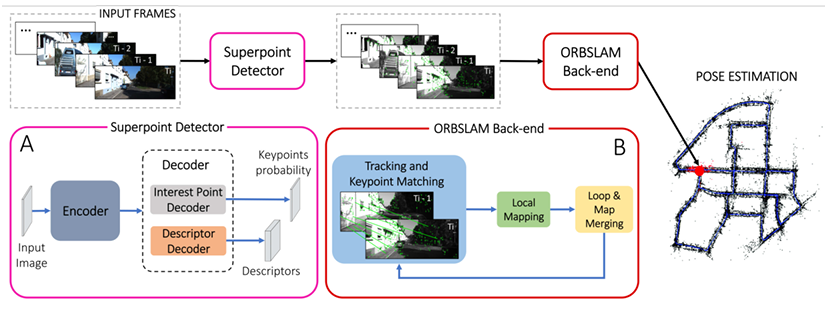
\includegraphics[width=0.8\textwidth]{images/superslam3.png}
    \caption{Integration of the Superpoint feature detector into the ORB-SLAM3 pipeline \cite{superslam3}.}
    \label{fig:superslam3_pipeline}
\end{figure}

\noindent\textbf{Advantages:} SUPERSLAM3 shows strong generalization across handheld, aerial, and automotive datasets without domain-specific weights, speeds up feature extraction relative to ORBSLAM3, and can outperform standard ORBSLAM3 in certain fast-motion indoor drone scenarios \cite{superpoint_slam3_2025,orbslam3}.

\noindent\textbf{Disadvantages:} It increases CPU memory use due to 256-element SuperPoint float descriptors, slows matching because it relies on $L_2$ distance rather than bit-wise ORB matching, and can suffer tracking drops or initialization failures in heavy motion blur or low-texture scenes \cite{superpoint_slam3_2025,superpoint,orbslam3}.

\subsubsection{SuperPoint SLAM3}
SuperPoint SLAM3 modifies the ORB-SLAM3 architecture by replacing handcrafted binary features with the \textbf{SuperPoint} network (DeTone et al., 2018) via the LibTorch C++ API. It utilizes 256-dimensional floating-point descriptors and implements Adaptive Non-Maximal Suppression (ANMS) to ensure uniform keypoint coverage across the image. The frontend matcher is rewritten to use Euclidean distance ($L_2$ norm) rather than the Hamming distance used for traditional binary features. \cite{orbslam3,superpoint_slam3_2025}

\begin{figure}[H]
    \centering
    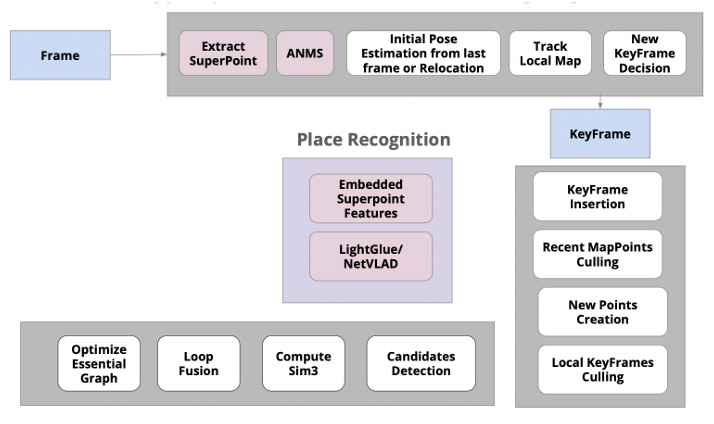
\includegraphics[width=0.8\textwidth]{images/superpoint_slam3.png}
    \caption{SuperPoint SLAM3 pipeline \cite{superpoint_slam3_2025}.}
    \label{fig:superpoint_slam3_pipeline}
\end{figure}


\begin{itemize}
    \item \textbf{Advantages:} This system reduces translational and rotational drift by providing more stable feature tracking. ANMS prevents keypoints from clustering in high-contrast areas, improving robustness in texture-sparse regions, while deep descriptors improve performance under illumination changes where standard ORB fails.
    \item \textbf{Disadvantages:} Floating-point descriptor matching is computationally heavier than binary operations, and storing 256-dimensional descriptors increases the memory footprint. Real-time operation typically requires a GPU, limiting deployment on ultra-low-power embedded devices.
\end{itemize}

\subsubsection{SELM SLAM3}
SELM-SLAM3 is designed for assistive navigation and is built using the ONNX Runtime C++ API to run \textbf{SuperPoint} (DeTone et al., 2018) and \textbf{LightGlue} (Lindenberger et al., 2023) natively without Python dependencies. It replaces standard projection-based tracking and Bag-of-Words matching with direct LightGlue inference, feeding current frames and local map points directly into the network to find correspondences. \cite{selm}

\begin{figure}[H]
    \centering
    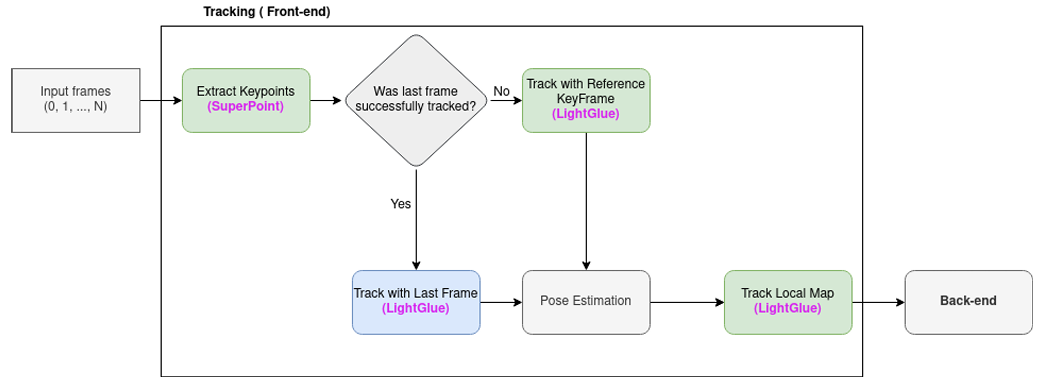
\includegraphics[width=0.8\textwidth]{images/selmslam.png}
    \caption{SELM-SLAM3 overview \cite{selm}.}
    \label{fig:selm_slam3_overview}
\end{figure}

\begin{itemize}
    \item \textbf{Advantages:} ONNX Runtime removes Python overhead, making the system easier to deploy and often faster than PyTorch-based hybrids. It offers strong robustness in low-texture scenes where heuristic matching fails and is optimized for erratic motion blur typical of wearable navigation aids.
    \item \textbf{Disadvantages:} Removing Bag-of-Words complicates loop closure and relocalization, requiring deep-learning replacements that increase compute. Despite using LightGlue, the end-to-end inference time for extraction and matching per frame remains higher than purely geometric approaches.
\end{itemize}

\subsubsection{Light-SLAM}
Light-SLAM addresses the lighting bottleneck of traditional methods by integrating a deep front-end using \textbf{SuperPoint} (DeTone et al., 2018) and \textbf{LightGlue} (Lindenberger et al., 2023) with a geometric backend. It incorporates an image enhancement module to restore gradient structures in low light and modifies the tracking thread to utilize LightGlue's adaptive depth mechanism, adjusting network inference complexity based on frame difficulty. \cite{lightslam,lightglue,superpoint}

\begin{figure}[H]
    \centering
    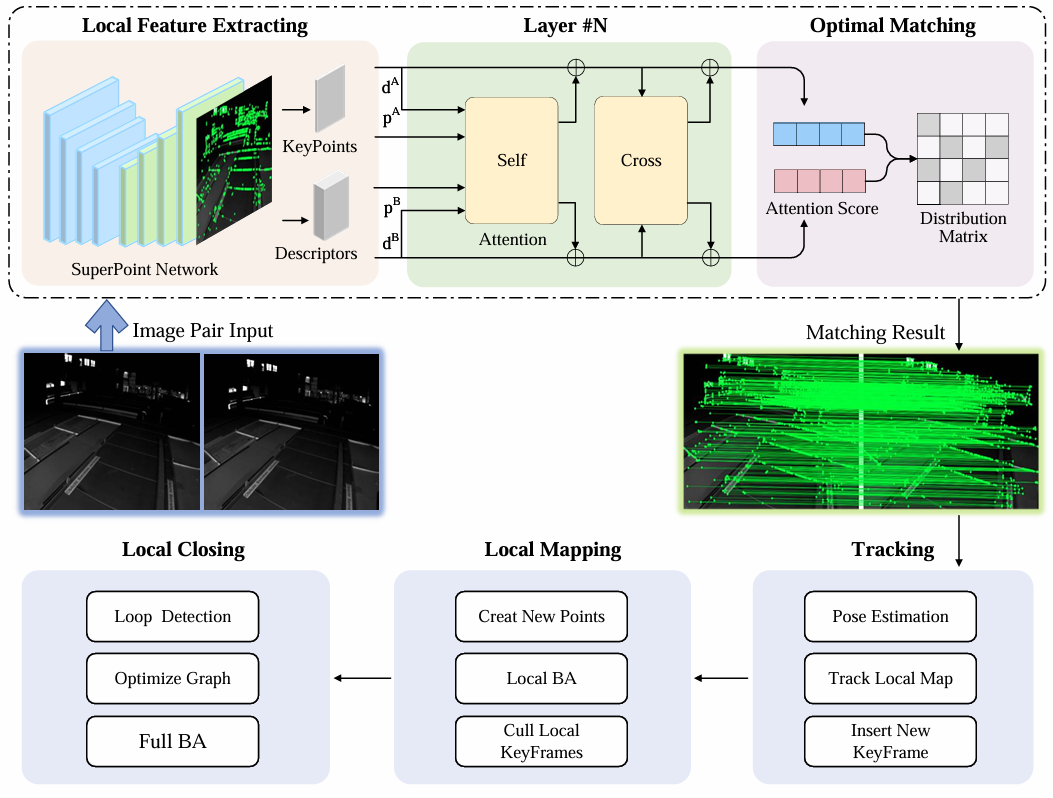
\includegraphics[width=0.8\textwidth]{images/lightslam.png}
    \caption{Light-SLAM architecture \cite{lightslam}.}
    \label{fig:lightslam_architecture}
\end{figure}


\begin{itemize}
    \item \textbf{Advantages:} Stable tracking in near-dark environments where traditional systems fail, with reduced compute on easy frames via early-stopping inference. Retains geometric accuracy of bundle adjustment while improving robustness under challenging illumination.
    \item \textbf{Disadvantages:} Still typically needs a CUDA-capable GPU, making it unsuitable for CPU-only platforms. Variable inference time can introduce jitter, which may affect control loops in autonomous robots.
\end{itemize}

\subsubsection{Deep-UAV SLAM}
Optimized for aerial robotics, Deep-UAV SLAM upgrades the ORB-SLAM3 front-end by integrating \textbf{SuperPoint} (DeTone et al., 2018) and \textbf{SuperGlue} (Sarlin et al., 2020) to handle bird's-eye views and rapid scale changes. A key innovation is retraining the Bag-of-Words vocabulary specifically for SuperPoint descriptors, enabling effective loop closure and relocalization. \cite{deepuav,superpoint,superglue}

\begin{figure}[H]
    \centering
    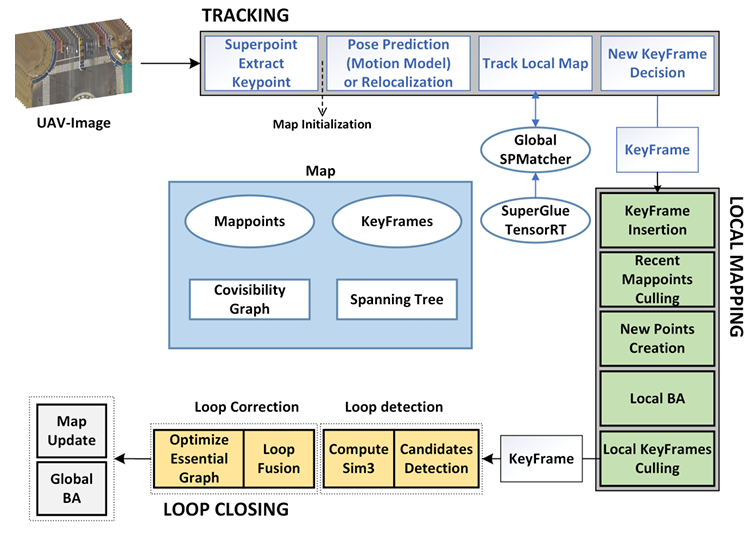
\includegraphics[width=0.8\textwidth]{images/deepuavslam.png}
    \caption{Deep-UAV SLAM pipeline \cite{deepuav}.}
    \label{fig:deepuavslam_pipeline}
\end{figure}

\begin{itemize}
    \item \textbf{Advantages:} Superior scale invariance for UAV altitude changes, improved robustness in dynamic outdoor aerial imagery, and a complete SLAM pipeline with functional relocalization and loop closure.
    \item \textbf{Disadvantages:} SuperGlue adds significant computational cost, typically requiring powerful edge AI hardware (e.g., Jetson-class). Building a Bag-of-Words vocabulary for continuous-space deep descriptors is complex and requires high-dimensional clustering.
\end{itemize}

\subsubsection{PCR-ORB}
PCR-ORB enhances the standard framework by integrating YOLOv8 for real-time semantic segmentation to identify and mask dynamic objects such as cars and people. It uses a CUDA-accelerated post-processing pipeline that refines the map by estimating the ground plane, removing sky artifacts, and enforcing temporal consistency on the point cloud. \cite{pcr}

\begin{figure}[H]
    \centering
    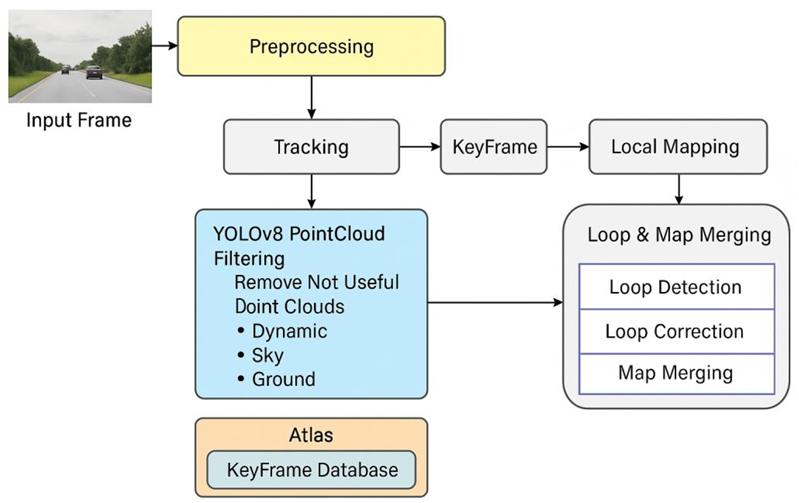
\includegraphics[width=0.8\textwidth]{images/pcrorb.png}
    \caption{PCR-ORB overview \cite{pcr}.}
    \label{fig:pcr_orb_overview}
\end{figure}

\begin{itemize}
    \item \textbf{Advantages:} Produces cleaner maps by reducing ghost trails from moving objects and removing sky artifacts. Improves robustness by avoiding feature lock-on to dynamic objects, adding semantic awareness to geometric SLAM.
    \item \textbf{Disadvantages:} Overhead can add latency in mostly static scenes with limited accuracy gains. Synchronizing heavy detection with the high-frequency tracking loop is challenging and can cause frame drops.
\end{itemize}

\noindent\textbf{Note:} The above method relies on SuperPoint for feature detection/description. \cite{superpoint}
\subsubsection{Summary}
\begin{table}[H]
\centering
\scriptsize % reduces font size
\caption{Comparison of Deep Learning-based VIO Algorithms}
\resizebox{\textwidth}{!}{%
\begin{tabular}{|p{1.5cm}|p{1.5cm}|p{1.5cm}|p{1.5cm}|p{4.5cm}|p{4.5cm}|}
\hline
\textbf{Algorithm} & \textbf{Deep Front-End} & \textbf{Deep Back-End} & \textbf{Primary Focus} & \textbf{Advantages} & \textbf{Disadvantages} \\
\hline

\hline
SUPER SLAM3 & Superpoint & Geometric SLAM + BoW (pre-trained) & Benchmark learned vs. handcrafted features &
\begin{itemize}[leftmargin=*, topsep=0pt, itemsep=0pt, parsep=0pt, partopsep=0pt]
  \item Generalizes across aerial, automotive, and handheld datasets with one pre-trained model.
  \item Faster keypoint/descriptor extraction than ORB.
\end{itemize} &
\begin{itemize}[leftmargin=*, topsep=0pt, itemsep=0pt, parsep=0pt, partopsep=0pt]
  \item Higher CPU memory from 256D float descriptors.
  \item Slower matching due to $L_2$ distance.
  \item Tracking degrades under heavy motion blur or low texture.
\end{itemize} \\
\hline

SuperPoint SLAM3 & SuperPoint & -- (geometric BA) & Robust feature tracking &
\begin{itemize}[leftmargin=*, topsep=0pt, itemsep=0pt, parsep=0pt, partopsep=0pt]
  \item Reduces translational/rotational drift via more stable learned features.
  \item Improved robustness under illumination changes; ANMS improves keypoint coverage in texture-sparse areas.
\end{itemize} &
\begin{itemize}[leftmargin=*, topsep=0pt, itemsep=0pt, parsep=0pt, partopsep=0pt]
  \item Heavier compute/memory than binary features due to floating-point descriptors and $L_2$ matching.
  \item Typically requires GPU for real-time performance on embedded platforms.
\end{itemize} \\
\hline

SELM-SLAM3 & SuperPoint + LightGlue & LightGlue correspondence inference & Robust matching (no BoW) &
\begin{itemize}[leftmargin=*, topsep=0pt, itemsep=0pt, parsep=0pt, partopsep=0pt]
  \item ONNX Runtime C++ deployment reduces Python overhead; often faster/easier to deploy than PyTorch hybrids.
  \item Strong robustness in low-texture scenes and under erratic motion blur.
\end{itemize} &
\begin{itemize}[leftmargin=*, topsep=0pt, itemsep=0pt, parsep=0pt, partopsep=0pt]
  \item Removing Bag-of-Words complicates loop closure/relocalization; deep replacements increase compute.
  \item End-to-end extraction+matching per frame can be slower than purely geometric approaches.
\end{itemize} \\
\hline

Light-SLAM & SuperPoint + LightGlue + image enhancement & Geometric backend & Low-light robustness &
\begin{itemize}[leftmargin=*, topsep=0pt, itemsep=0pt, parsep=0pt, partopsep=0pt]
  \item Stable tracking in near-dark environments; early-stopping inference reduces compute on easy frames.
  \item Retains geometric accuracy of bundle adjustment while improving robustness under challenging illumination.
\end{itemize} &
\begin{itemize}[leftmargin=*, topsep=0pt, itemsep=0pt, parsep=0pt, partopsep=0pt]
  \item Typically needs a CUDA-capable GPU; unsuitable for CPU-only platforms.
  \item Variable inference time may introduce jitter impacting real-time control loops.
\end{itemize} \\
\hline

Deep-UAV SLAM & SuperPoint + SuperGlue & Geometric SLAM + BoW (retrained) & Aerial robustness (scale/viewpoint) &
\begin{itemize}[leftmargin=*, topsep=0pt, itemsep=0pt, parsep=0pt, partopsep=0pt]
  \item Better scale invariance for UAV altitude changes; improved robustness for dynamic outdoor aerial imagery.
  \item Complete SLAM pipeline with functional relocalization and loop closure via retrained vocabulary.
\end{itemize} &
\begin{itemize}[leftmargin=*, topsep=0pt, itemsep=0pt, parsep=0pt, partopsep=0pt]
  \item SuperGlue adds significant computational cost (often needs Jetson-class hardware).
  \item Building BoW for high-dimensional deep descriptors is complex and expensive.
\end{itemize} \\
\hline

PCR-ORB & YOLOv8 (semantic masking) & Geometric SLAM + point-cloud refinement & Dynamic-object handling / clean maps &
\begin{itemize}[leftmargin=*, topsep=0pt, itemsep=0pt, parsep=0pt, partopsep=0pt]
  \item Cleaner maps by masking dynamic objects and removing sky/ground artifacts via post-processing.
  \item More robust tracking by avoiding features on moving objects (adds semantic awareness).
\end{itemize} &
\begin{itemize}[leftmargin=*, topsep=0pt, itemsep=0pt, parsep=0pt, partopsep=0pt]
  \item Added latency/overhead in mostly static scenes with limited gains.
  \item Synchronizing heavy detection with high-rate tracking is challenging; can cause frame drops.
\end{itemize} \\
\hline
\end{tabular}}
\label{tab:DL_VINS_comparison}
\end{table}



